\section{Numerische Ordinäre Differentialgleichungen}

  \subsection{Definitionen}
    Ordinäre DGL (ODE - ordinary differential equation)
    $$\boxed{y'(x) = f(x,y) \qquad\text{mit}\qquad y(x_0) = y_0}$$
    $f(x,y)$ wird auch als r.h.s. Funktion bezeichnet (right hand side).
    
    
    %\begin{minipage}{8cm}
      \subsection{Explizite Methoden}
      \label{sec:ode_explicit_methods}
      Es wird vorwärts in der Zeit gerechnet, was keine Solver braucht. Ansatz: Taylor-Approximation.
      Dies wird aber sehr schnell sehr aufwendig, da schnell höhere Ableitungen in mehrere 
      Dimensionen nötig werden.
      
      $$\boxed{y(x_0+h) = y(x_0) + \frac{h}{1!} y'(x_0) + \frac{h^2}{2!}y''(x_0) + \ldots + \frac{h^p}{p!}y^{(p)}(x_0) +\underset{\text{Restterm}}{\underbrace{ \frac{h^{p+1}}{(p+1)!}y^{(p+1)}(\xi)}}}$$
      
      Die Herleitung weiterer Ableitungen erfolgt mithilfe der Kettenregel: 
      $$\boxed{y''(x) = \frac{\partial f(x,y)}{\partial x} 1 + \frac{\partial f(x,y)}{\partial y}f(x,y)}$$
      Ableitungen bis zum dritten Grad sind hier aufgelistet (Immenser Rechenaufwand nötig):\\
      %\resizebox{\textwidth}{!}{
      \begin{tabular}{ll}
      	$y(x+h)=$&	$y(x)+\frac{f(x,y)}{1!}h+$\\
      				&$\frac{1}{2!}\left(\frac{\partial f(x,y)}{\partial x} 1+ \frac{\partial f(x,y)}{\partial y} f(x,y)\right)h^2+$\\
					&$\frac{1}{3!}\left(\frac{\partial^2f(x,y)}{\partial x^2} 1+2\frac{\partial^2f(x,y)}{\partial x\partial y}f(x,y)+\frac{\partial^2f(x,y)}{\partial y^2} f(x,y)^2+\left(\frac{\partial f(x,y)}{\partial y}\right)^2 f(x,y)+\frac{\partial f(x,y)}{\partial x}\frac{\partial f(x,y)}{\partial y}\right)h^3+\ldots+$\\
					&$\frac{1}{4!}y^{(4)}(x)h^4+\ldots+\frac{1}{p!}y^{(p)}(x)h^p+\underbrace{\frac{1}{(p+1)!}y^{(p+1)}(\xi)h^{p+1}}_{\text{Restterm}}$\\
      \end{tabular}\\
      %}
    %\end{minipage}
    %\hspace{8mm}
    %\begin{minipage}{11cm}
    %  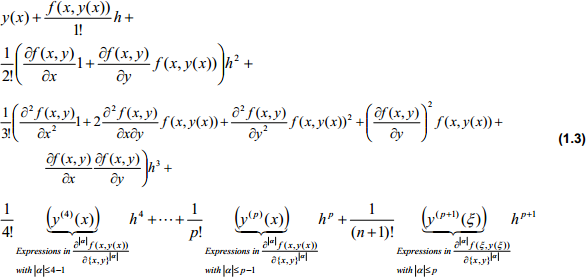
\includegraphics[width=10cm,trim=0cm 0cm 1.25cm 0cm,clip]{./bilder/ode_taylor_approx.png}
    %\end{minipage}\\
    
    
    
    
    \begin{minipage}{8cm}
      \subsubsection{Explizite Euler-Methode}
        Spezialfall der expliziten Methoden: Taylor mit Ordnung $p=1$. Relativ ungenaue Approximation,
        da hier die Ableitung pro Schritt unverändert bleibt. 
        
        Globaler Fehler: $\max_{0 \leq i \leq k} |y_i - y(x_i)|$ mit Anzahl Schritten $k$\\
        Lokaler Fehler: $y(x_n+h) - y_{n+1}$ wenn Initialwert des aktuellen Schritts is genau richtig
    \end{minipage}
    \hspace{8mm}
    \begin{minipage}{11cm}
      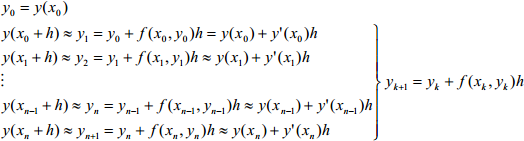
\includegraphics[width=10cm]{./bilder/ode_euler.png}
    \end{minipage}
      
    \subsubsection{Explizite Taylor-Methoden höherer Ordnung}
      Wenn $p > 1$ wird eine bessere Approximation erreicht. Allerdings steigt hier der rechnerische
      Aufwand enorm. Siehe Section \ref{sec:ode_explicit_methods} für Berechnung.
      
      
    \skriptsubsubsection{Explizite Runge-Kutta (RK) Methoden}{8}
      Es werden $s$ rekursive Stages $k$ definiert, welche zusammenaddiert die Taylor-Approximation ergeben.
      Hier ist $s=4$
      \begin{align*}
        k_1 &= f(x,y)\\
        k_2 &= f(x + m h, y+m h k_1)\\
        k_3 &= f(x + n h, y+n h  k_2)\\
        k_4 &= f(x + p h, y+p h k_3) 
      \end{align*}     
      $$y(x+h) \approx y(x) + a h k_1 + b h k_2 + c h k_3 + d h k_4 $$ 
      Im Gegensatz zum Skript (S. 10) sind die 
      $h$ nicht in den $k$-Definitionen enthalten, sondern erst in der finalen Formel. Mit den richtigen Nebenbedingungen (S. 11) 
      entspricht diese Formel dem Taylor Polynom bis zur Ordnung 4
      
      Mit der Gleichsetzung zu Taylor definieren die expliziten RK-Methoden ein 
      überbestimmtes Gleichungssystem mit 8 Gleichungen und 7 Unbekannten $m,n,p$ und $a,b,c,d$.
      
      Es gibt daher verschiedene \textbf{Lösungen}, die hier auch für die Ordnung $s=2$ und $s=4$ aufgeführt sind:\\
      \begin{tabular}{lll}
        Name der Lösungen & \# Stages ($s$) & Lösungen\\
        Heun & 2 & $a=b=\frac12$, $m=1$ ($n=p=c=d=0$)\\
        Explicit Midpoint & 2 & $a=0$, $b=1$, $m=\frac12$ ($n=p=c=d=0$)\\
        Klassische Runge-Kutta & 4 & $m=n=\frac12$, $p=1$, $a=d=\frac16$, $b=c=\frac13$
      \end{tabular}
      
      \vfill
      
      \newpage
      
    
    \skriptsubsubsection{Generelles Framework für Runge-Kutta Methoden (Butcher Tableaus)}{13}
      \begin{minipage}{6cm}
        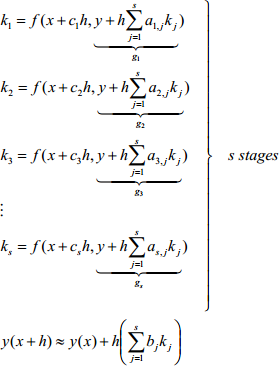
\includegraphics[width=5cm]{./bilder/ode_rungekutta_framework1.png}
      \end{minipage}
      \begin{minipage}{4.5cm}
        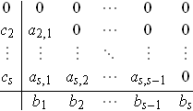
\includegraphics[width=3cm]{./bilder/ode_rungekutta_butcher.png}\\
        $\bm a$ = Aufteilung in $Y$\\
        $\bm b^T$ = Lösungen, durch Methode gegeben\\
        $\bm c$ = Aufteilung in $X$\\
        
        FSAL (First Same As Last) Spezialform:\\
        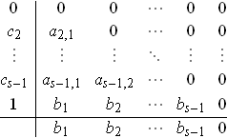
\includegraphics[width=3cm]{./bilder/butcher_fsal.png} 
      \end{minipage}
      \hspace{0.5cm}
      \begin{minipage}{9cm}
        Bedingungen (Für Explizite Methode): 
        \begin{liste}
          \item $c_i = \sum\limits_{j=1}^s a_{ij} = \sum\limits_{j=1}^{i-1} a_{ij}\,(i=2,\ldots,s)$
          \item $\sum\limits_{j=1}^s b_j = 1$
          \item $c_1=0$
          \item $a_{1j} = 0 \qquad 1\leq j\leq s $
          \item $a_{ij} = 0 \qquad j\geq i$
        \end{liste}
        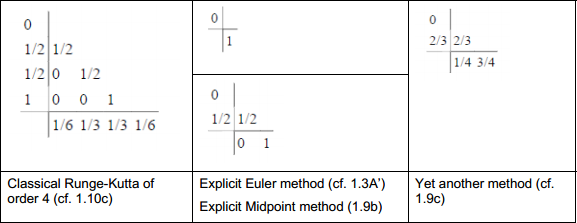
\includegraphics[width=8cm]{./bilder/ode_rungekutta_butcher_examples.png}\\
        Heun Methode (RK-2): $b_1 = b_2 = \frac{1}{2}; c_2=\frac{1}{2}; a_{2,1}=\frac{1}{2}$
      \end{minipage}
      
      
      
    \skriptsubsubsection{Adaptive Explizite Methoden}{17}
      Idee: Automatische Adaptierung der Step-Size $h$. Dies macht eine Definition des maximalen 
      Fehlers der Approximation nötig. Das \em Accuracy Goal \em ($ag$) 
      gibt die minimal übereinstimmende Anzahl Nachkommastellen an während
      das \em Precision Goal \em ($pg$) die Anzahl signifikanter Stellen des Resultats repräsentiert. 
      Der Toleranz-Paramter ist:
      $$\varepsilon = \varepsilon_a+ |y|\varepsilon_r=10^{-ag} + |y| 10^{-pg} \geq |e|.$$
      
      \subsubsubsection{Eingebettete Paare von expliziten Runge-Kutta Methoden}\\
        \begin{minipage}{5cm}
          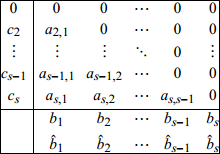
\includegraphics[width=4cm]{./bilder/ode_adaptive_butcher.png}
        \end{minipage}
        \begin{minipage}{13cm}
          Die Methode führt eine zweite Approximation, eine \em eingebettete Ordnung \em $\hat{p}$ 
          ein, welche für die Fehlerrechnung zuständig ist. Die \em primäre Ordnung \em $p$ wird 
          benötigt, um die Schrittweite zu berechnen. Meist ist $\hat{p} = p-1$.
          
          Das Butcher-Tableau wird dabei um eine Zeile der $b$-Zahlen erweitert.
        \end{minipage}\\
        
        Lokaler Fehler:
        $$e_n = y(x+h) - \hat{y}(x+h) = h_n \sum\limits_{j=1}^s (b_j - \hat{b}_j)k_j \Rightarrow 
        \Arrowvert e_n \Arrowvert = \left\Arrowvert h_n \sum\limits_{j=1}^s (b_j - \hat{b}_j)k_j \right\Arrowvert$$
          
        
        \begin{minipage}{7.5cm}
          Wenn bei aktuellem Schritt $\frac{\Arrowvert e_n \Arrowvert}{\varepsilon} < 1$, dann war die
          Schätzung von $h_n$ zu optimistisch und der Schritt muss mit kleinerer Schrittweite wiederholt
          werden (Reject). 
          
          Ansonsten wird fortgesetzt mit dem Update der Step-Size (Proceed): 
          $$h_{n+1} = h_n \left( \frac{\varepsilon}{\Arrowvert e_n \Arrowvert} \right)^{\frac{1}{\tilde{p}}}= 
          h_n \left( \frac{\Arrowvert e_n \Arrowvert}{\varepsilon} \right)^{-\frac{1}{\tilde{p}}}$$
          $$\varepsilon=\varepsilon_a+\varepsilon_r|y_n|
           \text{\qquad mit\quad} \tilde{p} = \min(p, \hat{p})+1$$
        \end{minipage}
        \hspace{0.5cm}
        \begin{minipage}{10.5cm}
          \subsubsubsection{Beispiel}\\
          \begin{tabular}{cccccc}
            \hline
            $x$ & $\bm y$ & $h_n$ & $\left( \frac{\Arrowvert e_n \Arrowvert}{\varepsilon} \right)^{-\frac{1}{\tilde{p}}}$ & $h_{n+1}$ & Status \\
            \hline
            $10$ & $[1, -1]^T$ & 1 & 0.4 & 0.4 & Reject\\
            10 & $[1,-1]^T$ & 0.4 & 1.5 & 0.6 & Proceed\\
            10.4 & $[0.420958, -1.40852]^T$ & 0.6 & 0.5 & 0.3 & Reject\\
            \hline
          \end{tabular}
        \end{minipage}
        
        
        
    \skriptsubsubsection{Stabilität von expliziten Methoden}{27}
      Globaler relativer Fehler darf nicht divergieren, d.h. muss beschränkt sein. 
      Da die Analyse mit zu untersuchender ODE wegen fehlender Kenntnis über die Lösung sehr schwierig
      ist, wird mit allgemeiner ODE gerechnet, dem Dahlquist Modell: 
      $$y' = A y \quad y(0) = 1 \qquad \text{mit } A = \Re\{A\} + j \Im\{A\} \in \mathbb{C}$$
      Dessen Lösung ist $y = e^{\Re\{A\} x} \left( \cos(\Im\{A\}x + j \sin(\Im\{A\} x) \right)$, also 
      eine Schwingung mit exponentieller Amplitude $e^{\Re\{A\} x}$ und Frequenz $\Im\{A\}$.
      
      Mit der zu untersuchenden Methode kann eine \em lineare Stabilitätsfunktion \em $F(z)$
      berechnet werden.
      
      \subsubsubsection{Beispiel} Anhand der Heun-Methode (RK-2) wird die Untersuchung gezeigt:
      \begin{align*}
        k_1 &= A y_k                                          & y_0 &= y(x_0) = y(0) = 1\\
        k_2 &= A(y_k + 1 h k_1) = A(y_k + Ah y_k) \qquad \Longrightarrow &
        y_{k+1} &= y_k \underbrace{\left(1 + hA + (hA)^2 \frac12\right)}_{F(hA) = F(z), \quad z=hA \in \mathbb{C}}
      \end{align*}
      Die lineare Stabilitätsfunktion kann jetzt auch so eingesetzt werden:
      $$y_{k+1} = \Big( | F(z) | \exp \big(j \arg(F(z))\big) \Big) y_k$$
      
      \begin{minipage}{10cm}
        Jetzt können drei Fälle unterschieden werden:
        \begin{liste}
          \item $\Re\{A\} < 0$: Die Amplitude der ODE wird exponentiell kleiner. Die Stabilitätsbedingung 
            verlangt, dass die approximierten Werte $y_k$ ($k=0,1,\ldots$) ebenfalls exponentiell 
            gedämpft werden. Daher und aus $y_{k+1} \propto | F(z) |$ folgt, dass $|F(z)| < 1$.
          \item $\Re\{A\} = 0$: Die Amplitude der ODE ist konstant 1. Die Stabilitätsbedingung 
            verlangt, dass die approximierten Werte $y_k$ ($k=0,1,\ldots$) ebenfalls konstant sind. 
            Daher und aus $y_{k+1} \propto | F(z) |$ folgt, dass $|F(z)| = 1$.
          \item $\Re\{A\} > 0$: Die Amplitude der ODE wird exponentiell grösser. Die Stabilitätsbedingung 
            verlangt, dass die approximierten Werte $y_k$ ($k=0,1,\ldots$) ebenfalls exponentiell 
            wachsen. Daher und aus $y_{k+1} \propto | F(z) |$ folgt, dass $|F(z)| > 1$.
        \end{liste}
        
        Die Fälle 2 und 3 bereiten keine Probleme (Bedingungen sind immer erfüllt), nur die erste Fall ist kritisch.
      \end{minipage}
      \hspace{1cm}
      \begin{minipage}{8cm}
        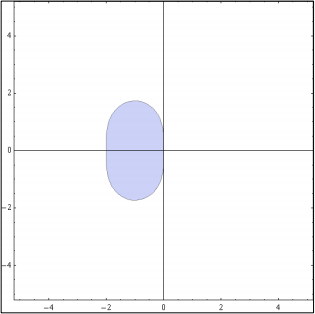
\includegraphics[width=6cm]{./bilder/ode_stability_heun.png}\\
        Fall 1 der Stabilitätsbedingung ($\Re\{A\} < 0$): \\
        $1 > |F(z)| = |1 + hA + \frac12 (hA)^2| \Rightarrow -2 < h \Re\{A\} < 0$.\\
        Fälle 2 und 3 sind in Abb. nicht berücksichtigt.
      \end{minipage}
      
      \vspace{1em}
      \subsubsubsection{Rekursive Formel} \formelbuch{29}
        Für das Stabilitätspolynom $F(z) = 1 + b_1 k_1(z) + \ldots + b_sk_s(z)$ existieren 
        rekursive Formeln:\\
        $k_1(z) = z, \qquad k_{j+1}(z) = z(1 + a_{j+1,1} k_1(z) + a_{j+1,2} k_2(z) + \ldots + a_{j+1,j} k_j(z))$
      
      \vspace{1em}
      \subsubsubsection{Schwäche der expliziten Methoden}: Stabilität!
    
    \skriptsubsubsection{Stiffness (Steifigkeit)}{33}
      Definition Stiffness = sehr schwierig (gemäss Wikipedia). Ungefähre Idee: Die expliziten 
      Methoden werden zu inakzeptabel kleinen Step-Sizes gezwungen (Computational complexity). 
      Dies trotz eigentlichen "`smoothen"' Oberflächen der Funktionen, die intuitiv nicht sehr 
      schwierig berechenbar sein sollten. \\
      
      Wenn Stabilitätsverletzungen (Stiffness) detektiert werden, soll zu 
      impliziten Verfahren (Blackbox-Solver) gewechselt werden, um dann mit non-Stiffness-Detektierung 
      zurück zu expliziten Verfahren umzustellen.\\
      
      Stiffness ist abhängig von:
      \begin{liste}
        \item Konkrete ODE
        \item Konkrete Schrittweite $h$
        \item Konkretes Verfahren (bspw. RK-4)
      \end{liste}
      
      \subsubsubsection{Stiffness Detektierung} 
        Voraussetzung: $c_{s-1} = c_s = 1$. Durch Testen von $\left|h \frac{\partial f(x,y)}{\partial y} \right|$ 
        auf die absolute Grenze der Stabilitätsregion kann
        Stiffness detektiert werden. Stiffness ist nicht erfüllt, wenn $|h \tilde{\lambda}|$ 
        ausserhalb des Stabilitätsbereich liegt.
        
        Beispiel explizite Runge-Kutta: 
        $$k_{s-1} = f(x+c_{s-1} h, \underbrace{y + h \sum\limits_{j=1}^s a_{s-1,j}k_j}_{g_{s-1}}) \qquad       
        k_{s} = f(x+c_{s} h, \underbrace{y + h \sum\limits_{j=1}^s a_{s,j}k_j}_{g_{s}}) \qquad 
        \Rightarrow \qquad \tilde{\lambda} = \frac{\Arrowvert k_s - k_{s-1} \Arrowvert}{\Arrowvert g_s - g_{s-1} \Arrowvert}$$
        
        $\tilde{\lambda}$ ist eine Schätzung für $f_y = \frac{\partial}{\partial y}f(x,y)$ z.B. $y'=x^4-25y^4=f(x,y)$ 
         und übernimmt die Rolle von $\Re \{A\}$ bei der Stabilitätsanalyse. 
        
        
  \skriptsubsection{Systeme von ODEs und ODEs höherer Ordnungen}{37}
    Systeme von ODEs werden in Vektor-Notation aufgeschrieben und wie üblich berechnet. 
    That's all.
    
  